%%%%%%%%%%%%%%%%%%%%%%%%%%%%%%%%%%%%%%%%%
% Programming/Coding Assignment
% LaTeX Template
%
% This template has been downloaded from:
% http://www.latextemplates.com
%
% Original author:
% Ted Pavlic (http://www.tedpavlic.com)
%
% Note:
% The \lipsum[#] commands throughout this template generate dummy text
% to fill the template out. These commands should all be removed when 
% writing assignment content.
%
% This template uses a Perl script as an example snippet of code, most other
% languages are also usable. Configure them in the "CODE INCLUSION 
% CONFIGURATION" section.
%
%%%%%%%%%%%%%%%%%%%%%%%%%%%%%%%%%%%%%%%%%%

%----------------------------------------------------------------------------------------
%	PACKAGES AND OTHER DOCUMENT CONFIGURATIONS
%----------------------------------------------------------------------------------------

\documentclass{article}

\usepackage{fancyhdr} % Required for custom headers
\usepackage{lastpage} % Required to determine the last page for the footer
\usepackage{extramarks} % Required for headers and footers
\usepackage[usenames,dvipsnames]{color} % Required for custom colors
\usepackage{graphicx} % Required to insert images
\usepackage{listings} % Required for insertion of code
\usepackage{courier} % Required for the courier font
\usepackage{hyperref}

\DeclareGraphicsExtensions{.png,.jpeg}

% Margins
\topmargin=-0.45in
\evensidemargin=0in
\oddsidemargin=0in
\textwidth=6.5in
\textheight=9.0in
\headsep=0.25in

\linespread{1.1} % Line spacing

% Set up the header and footer
\pagestyle{fancy}
\lhead{\hmwkAuthorName} % Top left header
\chead{\hmwkClass\ (\hmwkClassInstructor): \hmwkTitle} % Top center head
\rhead{\firstxmark} % Top right header
\lfoot{\lastxmark} % Bottom left footer
\cfoot{} % Bottom center footer
\rfoot{Page\ \thepage\ of\ \protect\pageref{LastPage}} % Bottom right footer
\renewcommand\headrulewidth{0.4pt} % Size of the header rule
\renewcommand\footrulewidth{0.4pt} % Size of the footer rule

\setlength\parindent{0pt} % Removes all indentation from paragraphs

%----------------------------------------------------------------------------------------
%	CODE INCLUSION CONFIGURATION
%----------------------------------------------------------------------------------------

\definecolor{MyDarkGreen}{rgb}{0.0,0.4,0.0} % This is the color used for comments
\lstloadlanguages{MATLAB} % Load Perl syntax for listings, for a list of other languages supported see: ftp://ftp.tex.ac.uk/tex-archive/macros/latex/contrib/listings/listings.pdf
\lstset{language=Matlab, % Use Perl in this example
        frame=single, % Single frame around code
        basicstyle=\small\ttfamily, % Use small true type font
        keywordstyle=[1]\color{Blue}\bf, % Perl functions bold and blue
        keywordstyle=[2]\color{Purple}, % Perl function arguments purple
        keywordstyle=[3]\color{Blue}\underbar, % Custom functions underlined and blue
        identifierstyle=, % Nothing special about identifiers                                         
        commentstyle=\usefont{T1}{pcr}{m}{sl}\color{MyDarkGreen}\small, % Comments small dark green courier font
        stringstyle=\color{Purple}, % Strings are purple
        showstringspaces=false, % Don't put marks in string spaces
        tabsize=5, % 5 spaces per tab
        %
        % Put standard Perl functions not included in the default language here
        morekeywords={rand},
        %
        % Put Perl function parameters here
        morekeywords=[2]{on, off, interp},
        %
        % Put user defined functions here
        morekeywords=[3]{test},
       	%
        morecomment=[l][\color{Blue}]{...}, % Line continuation (...) like blue comment
        numbers=left, % Line numbers on left
        firstnumber=1, % Line numbers start with line 1
        numberstyle=\tiny\color{Blue}, % Line numbers are blue and small
        stepnumber=5 % Line numbers go in steps of 5
}

% Creates a new command to include a perl script, the first parameter is the filename of the script (without .pl), the second parameter is the caption
\newcommand{\matlabscript}[2]{
\begin{itemize}
\item[]\lstinputlisting[caption=#2,label=matlab:#1]{../#1.m}
\end{itemize}
}

%----------------------------------------------------------------------------------------
%	DOCUMENT STRUCTURE COMMANDS
%	Skip this unless you know what you're doing
%----------------------------------------------------------------------------------------

% Header and footer for when a page split occurs within a problem environment
\newcommand{\enterProblemHeader}[1]{
\nobreak\extramarks{#1}{#1 continued on next page\ldots}\nobreak
\nobreak\extramarks{#1 (continued)}{#1 continued on next page\ldots}\nobreak
}

% Header and footer for when a page split occurs between problem environments
\newcommand{\exitProblemHeader}[1]{
\nobreak\extramarks{#1 (continued)}{#1 continued on next page\ldots}\nobreak
\nobreak\extramarks{#1}{}\nobreak
}

\setcounter{secnumdepth}{0} % Removes default section numbers
\newcounter{homeworkProblemCounter} % Creates a counter to keep track of the number of problems

\newcommand{\homeworkProblemName}{}
\newenvironment{homeworkProblem}[1][Problem \arabic{homeworkProblemCounter}]{ % Makes a new environment called homeworkProblem which takes 1 argument (custom name) but the default is "Problem #"
\stepcounter{homeworkProblemCounter} % Increase counter for number of problems
\renewcommand{\homeworkProblemName}{#1} % Assign \homeworkProblemName the name of the problem
\section{\homeworkProblemName} % Make a section in the document with the custom problem count
\enterProblemHeader{\homeworkProblemName} % Header and footer within the environment
}{
\exitProblemHeader{\homeworkProblemName} % Header and footer after the environment
\clearpage
}

\newcommand{\problemAnswer}[1]{ % Defines the problem answer command with the content as the only argument
\noindent\framebox[\columnwidth][c]{\begin{minipage}{0.98\columnwidth}#1\end{minipage}} % Makes the box around the problem answer and puts the content inside
}

\newcommand{\homeworkSectionName}{}
\newenvironment{homeworkSection}[1]{ % New environment for sections within homework problems, takes 1 argument - the name of the section
\renewcommand{\homeworkSectionName}{#1} % Assign \homeworkSectionName to the name of the section from the environment argument
\subsection{\homeworkSectionName} % Make a subsection with the custom name of the subsection
\enterProblemHeader{\homeworkProblemName\ [\homeworkSectionName]} % Header and footer within the environment
}{
\enterProblemHeader{\homeworkProblemName} % Header and footer after the environment
}

%----------------------------------------------------------------------------------------
%	NAME AND CLASS SECTION
%----------------------------------------------------------------------------------------

\newcommand{\hmwkTitle}{Assignment\ \#3} % Assignment title
\newcommand{\hmwkDueDate}{April 8,\ 2015} % Due date
\newcommand{\hmwkClass}{CS\ 4442B} % Course/class
\newcommand{\hmwkClassTime}{} % Class/lecture time
\newcommand{\hmwkClassInstructor}{Olga\ Veksler} % Teacher/lecturer
\newcommand{\hmwkAuthorName}{Kevin Brightwell} % Your name

%----------------------------------------------------------------------------------------
%	TITLE PAGE
%----------------------------------------------------------------------------------------

\title{
\vspace{2in}
\textmd{\textbf{\hmwkClass:\ \hmwkTitle}}\\
\normalsize\vspace{0.1in}\small{Due\ on\ \hmwkDueDate}\\
\vspace{0.1in}\large{\textit{\hmwkClassInstructor\ \hmwkClassTime}}
\vspace{3in}
}

\author{\textbf{\hmwkAuthorName}}
\date{} % Insert date here if you want it to appear below your name

%----------------------------------------------------------------------------------------

\begin{document}

\maketitle

%----------------------------------------------------------------------------------------
%	TABLE OF CONTENTS
%----------------------------------------------------------------------------------------

%\setcounter{tocdepth}{1} % Uncomment this line if you don't want subsections listed in the ToC

\newpage
\tableofcontents
\newpage

%----------------------------------------------------------------------------------------
%	PROBLEM 1
%----------------------------------------------------------------------------------------

% To have just one problem per page, simply put a \clearpage after each problem

\begin{homeworkProblem}

\matlabscript{applyMask}{Applies a linear mask}
\matlabscript{P1}{Use applyMask method}

\begin{figure}[htb!]
\centering
\includegraphics[width=\linewidth]{../swanFiltered.png}
\caption{Swan image after Sobel mask applied.}
\label{img:swanFiltered}

\end{figure}

\end{homeworkProblem}

%----------------------------------------------------------------------------------------
%	PROBLEM 2
%----------------------------------------------------------------------------------------

\begin{homeworkProblem}

\matlabscript{computeEngGradH}{Compute gradient energy for black and white image}
\matlabscript{P2}{Use computeEngGradH}

\begin{figure}[htb!]
\centering
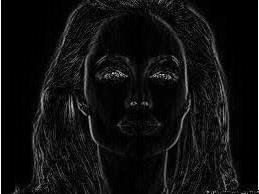
\includegraphics[width=\linewidth]{../faceEngG.jpg}
\caption{Energy image of `\textbf{face.jpg}'.}
\label{img:faceEngG}

\end{figure}

\end{homeworkProblem}

%----------------------------------------------------------------------------------------
%	PROBLEM 3
%----------------------------------------------------------------------------------------

\begin{homeworkProblem}

\matlabscript{computeEngColor}{Compute gradient energy for an RGB image}
\matlabscript{P3}{Use computeEngColor}

\begin{figure}[htb!]
\centering

\includegraphics[width=\linewidth]{../catEngC.png}
\caption{Energy image of `\textbf{cat.png}'.}
\label{img:catEngC}

\end{figure}

\end{homeworkProblem}

%----------------------------------------------------------------------------------------
%	PROBLEM 4
%----------------------------------------------------------------------------------------

\begin{homeworkProblem}

\matlabscript{removeSeamV}{Remove a vertical seam}
\matlabscript{addSeamV}{Add a vertical seam}
\matlabscript{seamV_DP}{Compute parameters for Dynamic Programming}
\matlabscript{bestSeamV}{Find a vertical seam through Dynamic Programming}
\matlabscript{reduceWidth}{Remove the lowest energy vertical seam}
\matlabscript{reduceHeight}{Remove the lowest energy horizontal seam}
\matlabscript{increaseWidth}{Add the lowest energy vertical seam}
\matlabscript{increaseHeight}{Add the lowest energy horizontal seam}
\matlabscript{intelligentResize}{Intelligently resize an image}

\matlabscript{P4}{Run several images through intelligent resize}

The energies used were Gradient and Colour, no masks or weights were used.  

\begin{figure}[htb!]
\centering
\includegraphics[width=\linewidth]{../catResized.png}
\caption{Rezied image of `\textbf{cat.png}', cost: $2.699556e+06$.}
\label{img:catResized}

\end{figure}

\begin{figure}[htb!]
\centering
\includegraphics[width=\linewidth]{../faceResized.jpg}
\caption{Rezied image of `\textbf{face.jpg}', cost: $5.508555e+05$.}
\label{img:faceResized}

\end{figure}

\begin{figure}[htb!]
\centering
\includegraphics[width=\linewidth]{../pigsResized.png}
\caption{Rezied image of `\textbf{pigs.png}', cost: $1.263304e+06$.}
\label{img:faceResized}

\end{figure}

\end{homeworkProblem}

%----------------------------------------------------------------------------------------
%	PROBLEM 5
%----------------------------------------------------------------------------------------

\begin{homeworkProblem}

\matlabscript{Code/forFG/segmentGC}{Segment graph-cut algorithm}

The energies used were Gradient and Colour, no masks or weights were used.  

\begin{figure}[htb!]
\centering
\includegraphics[width=\linewidth]{../pigsSeed.png}
\caption{Seed of pigs segmentation}
\label{img:pigsSeed}

\end{figure}

\begin{figure}[htb!]
\centering
\includegraphics[width=\linewidth]{../pigsSegment.png}
\caption{Segmentation output}
\label{img:pigsSegment}

\end{figure}

\begin{figure}[htb!]
\centering
\includegraphics[width=\linewidth]{../liftSeed.png}
\caption{Seed of lift segmentation}
\label{img:liftSeed}

\end{figure}

\begin{figure}[htb!]
\centering
\includegraphics[width=\linewidth]{../liftSegment.png}
\caption{Lift Segmentation}
\label{img:liftSegment}

\end{figure}



\end{homeworkProblem}

%----------------------------------------------------------------------------------------
%	PROBLEM 6
%----------------------------------------------------------------------------------------

\begin{homeworkProblem}

Incomplete.

\end{homeworkProblem}

%----------------------------------------------------------------------------------------
%	PROBLEM 7
%----------------------------------------------------------------------------------------

\begin{homeworkProblem}

\matlabscript{stereoCorrespondence}{Stereo Correspondence algorithm}
\matlabscript{P7}{Load stereo correspondence pairs}

\begin{figure}[htb!]
\centering
\includegraphics[width=\linewidth]{../teddy_disparity.png}
\caption{``Teddy'' stereo correspondence}
\label{img:teddyDisp}

\end{figure}

\begin{figure}[htb!]
\centering
\includegraphics[width=\linewidth]{../tsukuba_disparity.png}
\caption{``Tsukuba'' stereo correspondence}
\label{img:tsukubaDisp}

\end{figure}

\begin{figure}[htb!]
\centering
\includegraphics[width=\linewidth]{../venus_disparity.png}
\caption{``Venus'' stereo correspondence}
\label{img:venusDisp}

\end{figure}

\end{homeworkProblem}


%----------------------------------------------------------------------------------------

\end{document}